La figura \ref{fig:presupuesto_cliente} muestra el presupuesto del cliente.  En este presupuesto se han eliminado los detalles sobre los costes internos.

Para facilitar la comprensión del presupuesto por parte del cliente los costes internos se han dividido según los módulos con los que cuenta el sistema.  El peso de cada módulo se ha calculado dividiendo su tiempo de desarrollo entre el tiempo de desarrollo total del proyecto (exceptuando el tiempo destinado a tareas de pruebas, diseño y análisis).

Para la realización de este presupuesto se han utilizado dos nuevas variables:
\begin{itemize}
	\item El beneficio que se espera obtener del proyecto es de un 15\% sobre su coste total.
	\item Los impuestos aplicados corresponden a un IVA del 21\%
\end{itemize}

El coste total del proyecto incluyendo un beneficio del 15\% es de \EUR{41161,11}, tras aplicar los impuestos el coste final del proyecto resulta en \EUR{49804,94}.

\begin{figure}[h]
	\centering
	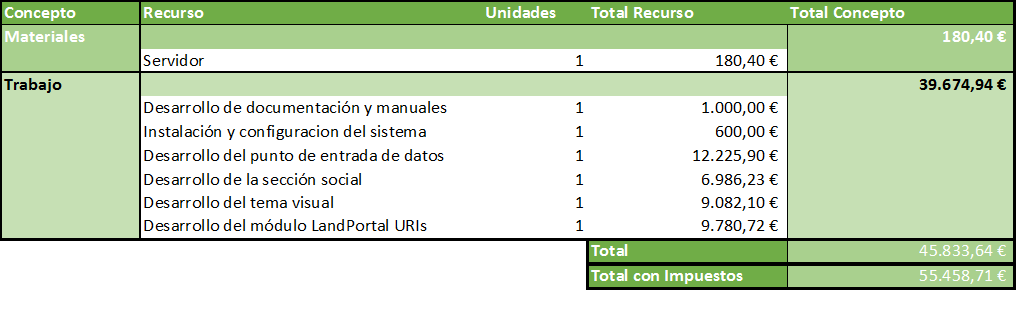
\includegraphics[width=\textwidth]{presupuesto/cliente}
	\caption{Presupuesto del cliente}
	\label{fig:presupuesto_cliente}
\end{figure}

\subsection{Condiciones del presupuesto}
A continuación se detallarán las condiciones a tener en cuenta por el cliente para aceptar este presupuesto:
\begin{itemize}
	\item El servidor utilizado será una instancia de \textit{Amazon EC2 m3.large} y se entregará totalmente configurado y con el sistema en marcha.  Una vez entregado el sistema será el cliente el encargado de pagar el coste de funcionamiento de dicho servidor.  Junto con el sistema también se entregarán unos \textit{scripts} que ejecuten la instalación automática del sistema.  Dichos \textit{scripts} requieren que el sistema resultante sea configurado manualmente.  En caso de que el cliente decidiera utilizar otro tipo de \textit{hosting} diferente al entregado la configuración no entrará en la garantía y tendría lugar como un proyecto nuevo.
	
	\item El código fuente del sistema estará disponible públicamente para su consulta en GitHub\footnote{Todos los repostorios que contienen el código del sistema están públicamente accesibles en \url{https://github.com/weso}}.  En caso de que el cliente decida modificar alguna parte del mismo, deberá crear previamente un \textit{fork} del repositorio que almacena el código antes de realizar alguna modificación.  El encargado de desplegar las modificaciones resultantes de \textit{forks} del sistema será en todo caso el propio cliente.
	
	\item Tras la entrega del sistema, el cliente contará con una garantía de un año.  Durante dicho periodo de garantía el cliente contará con actualizaciones para fallos de seguridad sin un coste añadido.  En cualquier caso, los desarrolladores no se harán responsables de los componentes que hayan sido modificados por el cliente tras su entrega.
	
	\item Los posibles bugs que no conlleven problemas de seguridad sólo se arreglarán de forma gratuita durante los tres meses posteriores a la entrega del sistema: Puesto que se ha efectuado un periodo de pruebas de aceptación en las cuales ha participado el propio cliente, este tipo de fallos se considerarán un fallo en dicho periodo de prueba del que será responsable el cliente.
\end{itemize}